\documentclass[12pt, a4paper]{article}
\usepackage{../../../myconfig} % Gọi file cấu hình từ ngoài gốc vào

% ==========================================
% BẮT ĐẦU NỘI DUNG TÀI LIỆU
% ==========================================
\begin{document}

% Truyền 3 tham số: {Nhãn cam} {Chữ to chính giữa} {Chữ ở góc phải Header}
\titlebox{Chủ đề: Hàm số}{BTDD min Max diện tích thể tích}{Hàm số: Min Max DT-TT}

\questionTrueFalse{0}{1}{Ông An cần xây dựng một bể chứa nước có dạng hình hộp chữ nhật không có nắp đậy để phục vụ cho việc tưới cây trong vườn. Do các điều kiện về diện tích vườn, ông An cần bể có thể tích là \( 24m^3 \), đáy bể có chiều dài gấp hai lần chiều rộng và chiều rộng không quá \( 4m \), biết rằng chi phí vật liệu xây dựng mỗi mét vuông diện tích bề mặt là \( 600\,000 \) đồng. Gọi \( x \, (m) \) là chiều rộng của bể, ta có \( 0 < x \leq 4 \). Khi đó:}{
    \textbf{a)} & Chiều cao của bể là \( \dfrac{12}{x^2} \, (m) \).
    & \textcolor{amberorange}{$\bigcirc$} & \textcolor{amberorange}{$\bigcirc$} \\ \hline
    
    \textbf{b)} & Tổng diện tích các mặt cần xây là \( 2x^2 + \dfrac{36}{x} \).
    & \textcolor{amberorange}{$\bigcirc$} & \textcolor{amberorange}{$\bigcirc$} \\ \hline
    
    \textbf{c)} & Để tổng chi phí vật liệu xây dựng là thấp nhất thì chiều cao của bể nước là \( h = \dfrac{2\sqrt[3]{18}}{3} \).
    & \textcolor{amberorange}{$\bigcirc$} & \textcolor{amberorange}{$\bigcirc$} \\ \hline
    
    \textbf{d)} & Ông An dự tính với ngân sách \( 24,5 \) triệu đồng thì sẽ đủ để ông có thể xây dựng bể chứa nước như mong muốn.
    & \textcolor{amberorange}{$\bigcirc$} & \textcolor{amberorange}{$\bigcirc$} \\
}

% --- CÂU 9 ---
\questionTrueFalse{0}{2}{Một tấm nhôm hình vuông cạnh 240 cm. Người ta cắt ở bốn góc của tấm nhôm đó bốn hình vuông bằng nhau, mỗi hình vuông có cạnh bằng \( x \) (cm), rồi gấp tấm nhôm lại như hình vẽ dưới đây để được một cái hộp không nắp.
\begin{center}
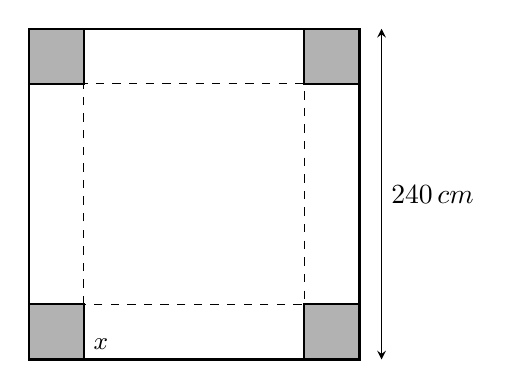
\begin{tikzpicture}[scale=0.35, >=stealth]
    % --- HÌNH 1: MẢNH CÁC TẤM BÌA PHẲNG ---
    % Khai báo kích thước tổng thể và cạnh cắt x
    \def\a{12}
    \def\x{2}
    
    % Tô màu xám cho 4 góc bị cắt
    \fill[gray!60] (0,0) rectangle (\x,\x);
    \fill[gray!60] (0,\a-\x) rectangle (\x,\a);
    \fill[gray!60] (\a-\x,0) rectangle (\a,\x);
    \fill[gray!60] (\a-\x,\a-\x) rectangle (\a,\a);
    \draw[thick] (0,0) rectangle (\x,\x);
    \draw[thick] (0,\a-\x) rectangle (\x,\a);
    \draw[thick] (\a-\x,0) rectangle (\a,\x);
    \draw[thick] (\a-\x,\a-\x) rectangle (\a,\a);
    % Vẽ biên ngoài hình vuông lớn
    \draw[thick] (0,0) rectangle (\a,\a);
    \draw[dashed] (\x,\x) rectangle (\a-\x,\a-\x);
   
    % Kí hiệu đoạn x ở góc
    \node at (\x, 0) [above right] {\small $x$};
    
    % Kí hiệu kích thước cạnh 12cm
    \draw[<->] (\a + 0.8, 0) -- (\a + 0.8, \a) node[midway, right] {$240\,cm$};
\end{tikzpicture}
\quad \quad \quad
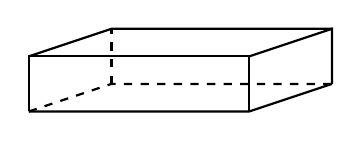
\begin{tikzpicture}[scale=0.35, >=stealth]
    % --- HÌNH 2: HÌNH HỘP CHỮ NHẬT 3D KHÔNG NẮP ---
    % Định nghĩa các điểm tọa độ mặt đáy
    \coordinate (A) at (0,0);
    \coordinate (B) at (8,0);
    \coordinate (C) at (11,1);
    \coordinate (D) at (3,1);
    
    % Chiều cao hộp h
    \def\h{2}
    
    % Các điểm mặt trên
    \coordinate (A1) at (0,\h);
    \coordinate (B1) at (8,\h);
    \coordinate (C1) at (11,3);
    \coordinate (D1) at (3,3);
    
    % Vẽ các nét khuất (nét đứt phía sau)
    \draw[dashed, thick] (A) -- (D) -- (C);
    \draw[dashed, thick] (D) -- (D1);
    
    % Vẽ các nét thấy phía trước và mặt trên mở
    \draw[thick] (A) -- (B) -- (C);
    \draw[thick] (A) -- (A1) -- (B1) -- (B);
    \draw[thick] (B1) -- (C1) -- (C);
    \draw[thick] (A1) -- (D1) -- (C1);
    
\end{tikzpicture}
\end{center}
}
{
    \textbf{a)} & Thể tích khối hộp nhận được khi tính theo \( x \) là  
    \(V = x(240 - 2x)^2.\)
    & \textcolor{amberorange}{$\bigcirc$} & \textcolor{amberorange}{$\bigcirc$} \\ \hline
    
    \textbf{b)} & Khi \( x = 20 \, cm \) thì thể tích của khối hộp nhận được là \( 8 \, m^3 \).
    & \textcolor{amberorange}{$\bigcirc$} & \textcolor{amberorange}{$\bigcirc$} \\ \hline
    
    \textbf{c)} & Để hộp nhận được có thể tích lớn nhất thì \( x = 60 \, cm \).
    & \textcolor{amberorange}{$\bigcirc$} & \textcolor{amberorange}{$\bigcirc$} \\ \hline
    
    \textbf{d)} & Hộp nhận được có thể tích lớn nhất là \( 1024 \, dm^3 \).
    & \textcolor{amberorange}{$\bigcirc$} & \textcolor{amberorange}{$\bigcirc$} \\
}

% --- CÂU 24 ---
\questionShortAnswer{0}{3}{Một người nông dân có 18 000 000 đồng để làm một hàng rào hình chữ \( E \) dọc theo một con sông bao quanh hai khu đất trồng rau có dạng hai hình chữ nhật bằng nhau (hình vẽ). Đối với mặt hàng rào song song với bờ sông thì chi phí nguyên vật liệu là 60 000 đồng/mét, còn đối với ba mặt hàng rào song song nhau thì chi phí nguyên vật liệu là 20 000 đồng/mét, mặt giáp với bờ sông không phải rào. Tìm diện tích lớn nhất của hai khu đất thu được sau khi làm hàng rào (đơn vị: ha).

\begin{center}
\begin{tikzpicture}[>=latex, scale=0.8]
    \begin{scope}[xshift=0cm, yshift=0cm]
        \node[anchor=south west, inner sep=0] at (0,0) {
            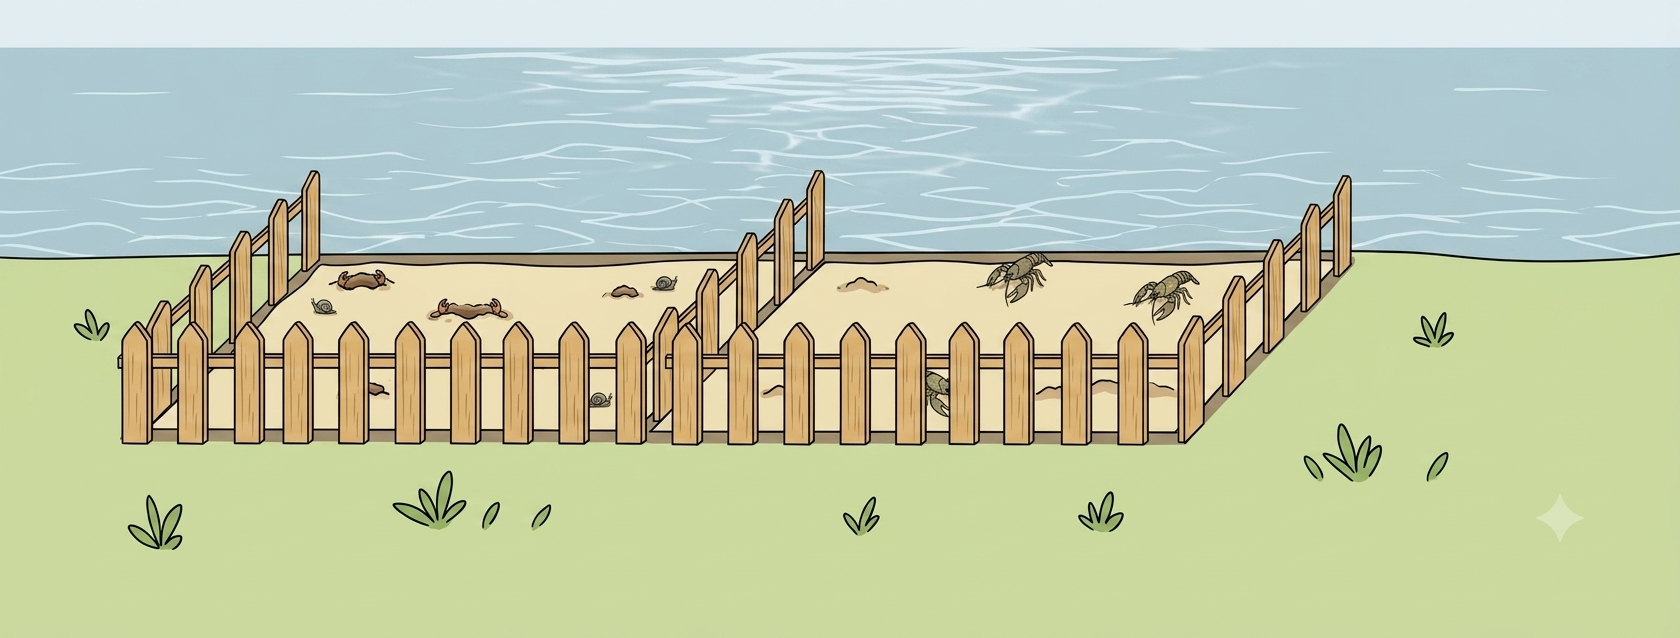
\includegraphics[width=5cm]{../images/HangRao.png}
        };
    \end{scope}
\end{tikzpicture}
\end{center}}


% --- CÂU 13 ---
\questionShortAnswer{0}{4}{Anh Tú dự định làm một cái thùng đựng nước hình trụ bằng nhôm có nắp đậy có thể tích \( 30 \, m^3 \). Chi phí làm mỗi \( m^2 \) đáy là 200 000 đồng, mỗi \( m^2 \) nắp là 100 000 đồng và mỗi \( m^2 \) mặt xung quanh là 150 000 đồng. Để chi phí làm thùng là thấp nhất thì anh Tú nên làm chiếc thùng với chiều cao là bao nhiêu mét? (Xem độ dài của tấm nhôm là không đáng kể, kết quả làm tròn đến hàng phần trăm).}


\end{document}